\documentclass[10pt]{article}

\usepackage{amsmath} \usepackage{amssymb} \usepackage{anysize}
\usepackage{amsthm} \usepackage{commath} \usepackage{float}
\usepackage{listings} \usepackage{graphicx}

\let\emptyset\varnothing

\marginsize{1in}{1in}{1in}{1in}
\title{\vspace{-2em}Site level interactions between intensive blood pressure management and
  adverse outcomes in SPRINT}
\author{Stats For Good}
\date{\today}

\begin{document} \maketitle

\begin{abstract}
  The SPRINT study defines a number of subgroup analyses to test for
  interactions between the treatment and other variables, for which they find no
  significance. With respect to the primary outcome, we find nonsignificance
  for most relevant baseline variables. Beyond this, we argue that interactions
  between treatment site and the intensive treatment are interesting to
  consider, and use statistical analysis to demonstrate there are plausible
  interactions that deserve further investigation. 
\end{abstract}

\section{Covariate interactions}
\subsection{Methods}
We were interested in studying any interactions between intensive
versus standard treatment and patient covariates on the incidence of
adverse events during the study. This was fit with a Cox proportional
hazards model with race, gender, BMI, smoking status, and medications
(aspirin and statins) and pairwise interactions with the intensive
treatment. 

Further, we investigated the possibility that subgroups defined via specific
thresholds of baseline covariates may have stronger interactions with the
treatment variable. To this end, we fit an honest decision tree (TODO: add
citation to Athey and Imbens) with the binary outcome of incidence of primary
CVD within 5 years.

\subsection{Results}
Corresponsing network IDs and the number of individuals in reidentified networks
can be found on our GitHub page; also, state-level American Community Survey (ACS)
data for the sites listed in the protocol's Supplementary Appendix. To associate
sites with the most probable network, we compared site size and demographic
characteristics from the baseline.csv with American Community Survey
(ACS) data.  For example, we assumed sites with a high proportion of males
woere likely to be in the VA network, large sites with a high proportion of whites
were in the Ohio network, sites with a high proportion of hispanics
were in UAB network and sites with a high relative median age were in the SouthEast
network.  NA was used as a placeholder for all sites that were not identified.

No interactions were significant for primary outcomes (P > 0.1) or severe
adverse events (P > 0.1). In the fitted causal tree, BMI was the only variable
considered in the top two layers of the tree, so we considered the average
treatment effect of the intensive treatment in each decile of BMI, included in
Figure (TODO: make into figure), in which no clear trend is apparent. 

\includegraphics[width=3.5in]{sae_bmi_interaction.eps}

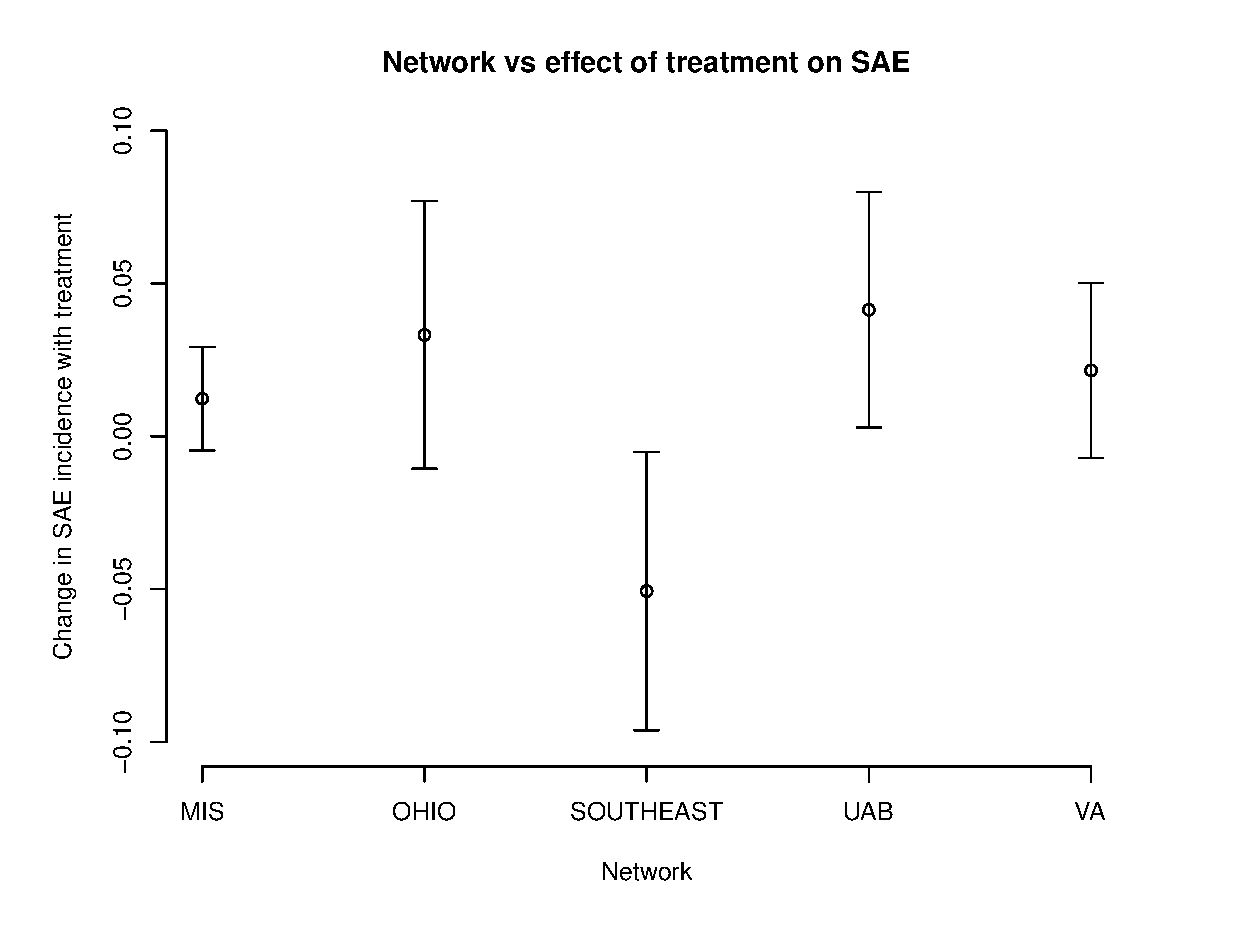
\includegraphics[width=3.5in]{sae_network_interaction.eps}

\section{Site specific outcomes}
\subsection{Methods}
TODO: include explanation of how networks were identified.
Among the networks identified, we tested for interactions between the provider
network as a categorical factor, and the intensive treatment against adverse
events as the outcome. All individuals who were a part of the study but not one
of the five identifiable networks were included as a baseline factor. We fit a
multivariate proportional hazards Cox model to these data, and looked for
significance at the $P = 0.1$ and $P=0.05$ levels.

\subsection{Results}
NA is used as a placeholder for all sites that were not identified $(n = 5,285)$. $844$ people were from sites identified in the Ohio network, 733 in the Southeast, 489 in UAB, and 1970 in the VA.

Among these sites, the interaction between the intensive treatment and the
Southeast network was found to be significant at $P = 0.068$ ($Z =
-1.823$). That is, individuals in the Southeast network were less
likely to have a severe adverse event mediated by the intensive versus
standard treatment than the average individual in the study.

\subsection{Conclusions}
The significance for the network level interactions found was inconclusive,
however it warrants further investigation. As the study was not powered to
consider these geographic interactions with respect to adverse events, the data
derived from the SPRINT study provide an exploratory look at considering these
interactions.

As the baseline covariates did not have significant interactions with
the treatment for adverse events, the potential for demographic
differences between populations to explain the differences in the
effect of intensive treatment on adverse outcomes. Potential
explanations include variation in the class of secondary hypertensive
medications prescribed among different networks, and factors
influencing regional noncompliance.

The first step would be analysis with the un-anonymized site
information, followed by a RCT powered to understand how demographic and
geographic factors mediate the adverse effects of intensive blood pressure
management.

\end{document}

\bibliographystyle{plain}
\bibliography{nejm-sprint}
